\documentclass[../main.tex]{subfiles}
\begin{document}
    \chapter{Research Context}\label{ch:inference_design_context}

	This chapter describes the research context.
    In section \ref{sec:types} we explain more about our defined types.
    The relation between the types are described in \ref{sec:type_hierarchie}.
    Section \ref{sec:implementation_context} explains in which context the research is executed.
    
	\section{Types}\label{sec:types}
	The basis types in PHP are integers, floats, booleans, strings, arrays, resources and objects.
	PHP has a similar class inheritance structure and interface implementation as Java.
    The main difference is that in PHP all class are \texttt{public} and that inner classes are not allowed in PHP. 
    \\
	Because PHP has no explicit type system, we define our own type system for PHP.
	In the Rascal code below in Rascal \ref{fig:rascal_typesymbols} you can see our defined types.
	Here we define the \texttt{TypeSymbol} data type in Rascal with our defined types as possible values.
	A brief description of all the defined types are listed below.
	\begin{program}
    \begin{rascal}
\CAT{Keyword}{module} lang::php::m3::TypeSymbol
 
\CAT{Keyword}{data} TypeSymbol
  = \textbackslash{}any()\footnotemark                         \CAT{Comment}{// unknown, can be any of the types below}
  | arrayType(TypeSymbol arrayType) \CAT{Comment}{// array of a type}
  | booleanType()                   \CAT{Comment}{// boolean values}
  | classType(\CAT{Keyword}{loc} decl)             \CAT{Comment}{// a specific class}
  | floatType()                     \CAT{Comment}{// float, double or real}
  | integerType()                   \CAT{Comment}{// integer numbers}
  | interfaceType(\CAT{Keyword}{loc} decl)         \CAT{Comment}{// a specific interface}
  | numberType()                    \CAT{Comment}{// a float or integer}
  | nullType()                      \CAT{Comment}{// empty or undefined value}
  | objectType()                    \CAT{Comment}{// any class type}
  | resourceType()                  \CAT{Comment}{// a build-in type}
  | scalarType()                    \CAT{Comment}{// any number, string, resource or boolean}
  | stringType()                    \CAT{Comment}{// text values}
  ; 
    \end{rascal}
	\caption{TypeSymbol definitions in Rascal}
	\label{fig:rascal_typesymbols}
	\end{program} 
	\footnotetext{any is escaped with a backslash because it is a reserved keyword.}      
    
    \paragraph{any} 
    As you can see in the comments in the code above, Rascal \ref{fig:rascal_typesymbols}, \texttt{any()} represents the combination of all possible types. 
    This type will be used for mixed and unknown types, for example when variables are used, but are never defined.
    
    \paragraph{arrayType}
    The type \texttt{arrayType(TypeSymbol arrayType)} is a recursive declaration.
    The argument of the type is the type of the array. 
    For example, an array of strings is declared as \texttt{arrayType(stringType())} and for an unknown array the type is \texttt{arrayType(\textbackslash{}any())}.
    
    \paragraph{booleanType}
    The type \texttt{booleanType()} is the type for boolean values.
    Boolean values are \texttt{true} and \texttt{false}.
    
    \paragraph{classType}
    The type \texttt{classType(loc decl)} represents a specific class.
    The argument is the declaration, which represents the logical name of the class. 
    An example of the \texttt{Exception} class is \texttt{classType(|php+class:///exception|)}.
    
    \paragraph{floatType}
    Floating point numbers, represented as floats, reals, and doubles are defined by the \texttt{floatType()}.
    Example are \texttt{1.234}, \texttt{1.2e3}, and \texttt{7E-10}.
    
    \paragraph{integerType}
    Integers are whole numbers in decimal, hexadecimal, octal or binary notation.
    The \texttt{integerType} values can be positive or negative.
    
    \paragraph{interfaceType}
    The \texttt{interfaceType(loc decl)} represents a specific interface.
    Interfaces can be provided as type hints.
    
    \paragraph{numberType}
    The type \texttt{numberType()} covers the \texttt{integerType()} and \texttt{floatType()}.
    Because of type coercion in PHP, these types can be easily mixed.
    
    \paragraph{nullType}
    The type \texttt{nullType()} is used for the value \texttt{null}.
    
    \paragraph{objectType}
    The type \texttt{objectType()} is the parent type for all class types.
    This type represent the object type and could also been written as \texttt{classType(|php+class:///object|)}.
    
    \paragraph{resourceType}
    The type \texttt{resourceType()} represents the build-in PHP resource type.
    Various function return the resourceType from build-in PHP functions.
    
    \paragraph{scalarType}
    The type \texttt{scalarType()} is the generic type for \texttt{resourceType()}, \texttt{booleanType()}, \texttt{numberType()}, and \texttt{stringType()}.
    
    \paragraph{stringType}
    The type \texttt{stringType()} represents strings, a sequence of characters.
    
    % layout hack!
    \pagebreak
    
    \section{Type hierarchie}\label{sec:type_hierarchie}
    
    As described in some of the previous descriptions, types can relate to other types.
    The full relation schema of the types is shown in figure \ref{fig:type_hierarchie}.
    In this diagram the \texttt{-Type} postfix is omitted to save space.
    We speak of \textbf{subtypes} when the types are descendant of the given type.
    The subtypes of the root node \texttt{any} are \texttt{scalarType}, \texttt{arrayType}, and \texttt{objectType}.
    
    \begin{figure}[H]
        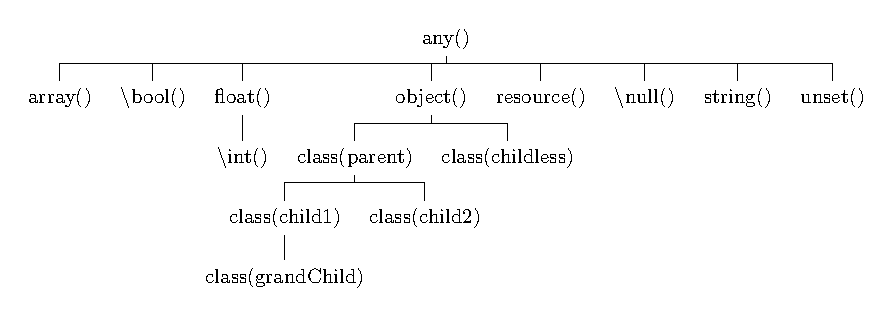
\includegraphics{Diagrams/Subtypes.pdf}
        \caption{Type hierarchy}
        \label{fig:type_hierarchie}
    \end{figure}
    

    The \textit{scalar type} is the super type for the non-complex types \texttt{resourceType}, \texttt{booleanType}, \texttt{numberTypes}, and \texttt{stringType}.
    These types can in practise be combined because of coercion.
    If they are used mixed up, they will be classified as scalar types.
    
	The \textit{array type} in the subtype diagram is the most generic type of array, the array of any type.
	We have omitted the other array types to reduce complexity of the hierarchy.
	The array type is a recursive type and can go to infinite depth.
 
    % show three images next to each other
    \begin{figure}[H]
    \begin{subfigure}[b]{.33\textwidth}
      \begin{center}
      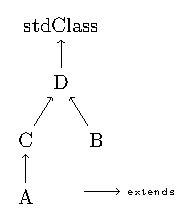
\includegraphics[scale=1]{Diagrams/Inheritance_example.pdf}
      \caption{Inheritance relation}
      \label{fig:subtype}
      \end{center}
    \end{subfigure}
    \begin{subfigure}[b]{.33\textwidth}
      \begin{center}
      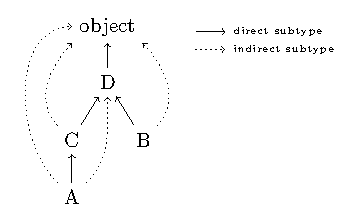
\includegraphics[scale=1]{Diagrams/Subtypes_example.pdf}
      \caption{Subtype relation}
      \label{subtype_tc}
      \end{center}
    \end{subfigure}
    \begin{subfigure}[b]{.33\textwidth}
      \begin{center}
      \lstinputlisting[nolol=true,xleftmargin=20pt,xrightmargin=20pt,language=PHP]{src/php/inheritance.php}
      \caption{Inheritance in PHP}
      \label{subtype_code}
      \end{center}
    \end{subfigure}
    \caption{Relation of subtypes among classes}
    \label{fig:subtypes_classes}
    \end{figure}

	The \textit{object type} is the most generic object type, which represents the \texttt{stdClass} in PHP.
    The class inheritance relation in PHP is a \gls{reflexive transitive closure} relation.
    A class extension of \textbf{\texttt{class A}} on \textbf{\texttt{class C}} will define \textbf{\texttt{class A}} as a subtype of \textbf{\texttt{class C}} in our analysis, as you can see in figure \ref{fig:subtypes_classes}.
    If a class does not extend another class, it will implicitly extend the \gls{stdClass} class.
    You can see that this happens with \textbf{\texttt{class D}} in the example.
    The \textbf{\texttt{stdClass}} is represented as the type \textbf{\texttt{object()}} in our analysis.

    % layout hack!
    \pagebreak
    
    \section{Research context}\label{sec:implementation_context}
    In order to let our research take place, we need to make sure that some environment variables are constant.
    
    \paragraph{Program correctness}
    In order to be able to execute this research we assume that the programs are correct and works as intended.
    This is needed to be able to reason about the programs we analyse, without having to question wether the program works as intended.
    
    \paragraph{File includes}
    In this research we assume that all PHP file are included during runtime within the project folder. 
    When a PHP system is constructed of classes with namespaces, the files will be logically loaded using PHP's autoloader.
    Because most recent systems use namespaces, we will assume that all files are included.
    For our experiment we are sure that all chosen projects comply to this.
    
    \paragraph{Register globals}
    Register globals allows variables to be magically be created from GET and POST values.
    Since it is discouraged to use this setting, we will assume that all software products have this setting disabled.
    This feature is disabled by default in version 4.2 and has been completely removed in version 5.4.
    
    \paragraph{PHP warnings}
    For this research we will ignore all warnings.
    Warnings do not alter the behaviour of the program.
    In a most production environment these warnings are suppressed and will not change the behaviour of the program.
    We do take fatal errors into account, which lead to runtime errors.
    
    \paragraph{Flow insensitive}
    Our analysis is intra-procedural flow-insensitive, which means that we don't take the order of statements into account within a function or method scope.
    We do assume type consistency within a scope.
        
\end{document}